With the confirmation of the overall project goal and the set of aims for research, it is vital to consider the overall background information consisting of highly specialised technical subject theory to develop a rigorous theoretical basis for the project design and experimental work before considering project objectives and intended approach.

\subsection{Computing Platforms}
Field Programmable Gate Arrays (FPGAs) are semiconductor devices based around a matrix of configurable logic blocks (CLBs) connected via programmable interconnects, enabling the hardware reprogramming to desired application or functionality requirements after manufacturing \cite{WhatFPGAField}. The flexibility of FPGA-based systems allows for very diverse and capable solutions, with their parallelism allowing for efficient computation and re-programmability for efficient use of hardware without the need to dedicate hardware for a task that may only last a few seconds \cite{villalpandoReconfigurableMachineVision2010}. Unlike FPGAs, CPUs compute sequentially, breaking algorithms into operations by sequence, thus limiting execution to one operation at a time \cite{alexliangBoostingMachineVision2016}.

The Raspberry Pi (RPi) company has been designing single-board and modular computers built on the Arm architecture and running the Linux operating system since 2012, with a mission to put high-performance, low-cost, general-purpose computing platforms in the hands of enthusiasts and engineers worldwide \cite{raspberrypiRaspberryPiUs}. The regular RPi product series features single-board computers powered by Broadcom-built Arm Cortex-based multicore processors. Perfect for a non-FPGA, CPU-based route, the newer RPi models implement various features such as built-in RAM up to 8GB, a dedicated GPU and video decoder, HDMI output interfaces, dual-band WiFi with Bluetooth capabilities, a Gigabit Ethernet interface, USB 3.0 and 2.0 ports, MIPI-compatible serial interfaces for cameras and displays, and an array of 40 GPIO pins \cite{raspberrypiltdBuyRaspberryPi, raspberrypiltdBuyRaspberryPia}.

\subsection{Specialised Light Source}
The Digital Light Processing (DLP) chipset, created by Larry Hornbeck of Texas Instruments in 1987, consists of a Digital Micromirror Device (DMD) that houses millions of reflective aluminium mirrors, usually a few microns wide \cite{DigitalLightProcessing2024, HowDoesDLP}. The DMD is a Micro-Opto-Electro-Mechanical System (MOEMS) Spatial Light Modulator (SLM) that uses digital signals to control the angle of each mirror, enabling the modulation and attenuation of an incident light beam \cite{DLP4500DigitalMicromirror}.

\begin{figure}[h]
    \centering
    \begin{subfigure}{.4\textwidth}
        \centering
        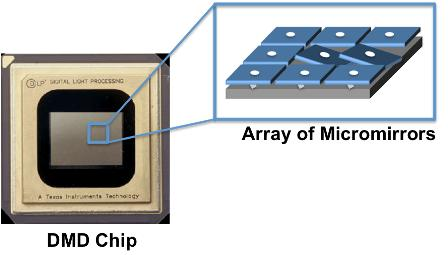
\includegraphics[width=1\linewidth]{assets/dmd-chip.jpg}
        \caption{}
        % \label{subfig:dmd_chip}
    \end{subfigure}
    % \hfill
    \qquad
    \begin{subfigure}{.4\textwidth}
        \centering
        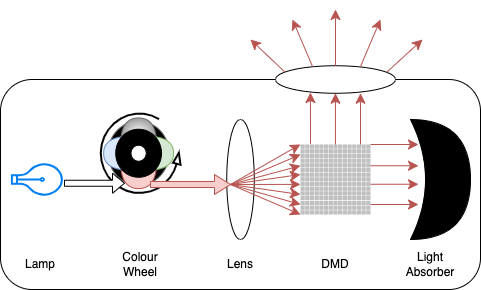
\includegraphics[width=1\linewidth]{assets/dlp-projector.png}
        \caption{}
        % \label{subfig:dlp_projector}
    \end{subfigure}
    \caption{(a) An illustration of the microscopic mirror array within a DMD chip \cite{HowDoesDLP}. (b) A cross-section illustrating the internals of an example projector utilising DLP technology.}
    \label{fig:dmd_dlp}
\end{figure}

As \cite{HowDLPProjector} explains the intricacies and Figure \ref{fig:dmd_dlp} illustrates, a DLP projector implements this specialised technology: The beam of a high-intensity white lamp directs into a spinning colour-tinted lens wheel consisting of red, green, and blue, and a clear lens for a white lamp pass-through. An internal lens diffracts the coloured beam incident into the DMD, with the angle and time spent in each microscopic mirror controlling the individual pixel colour and intensity. The DMD directs the desired beams of each pixel into the diffraction lens to exit the projector. The DMD will not actuate for undesired pixel beams, thus sending the beam into a light-absorbent region to prevent leakage and image distortion.

\subsection{Specialised Camera}
The cameras in most traditional and consumer-grade electronic devices, such as phones, all employ a CMOS sensor with a rolling shutter. While these sensors are smaller and much cheaper, they cause distortion effects when capturing fast-moving subjects due to their line-by-line scan image-capturing characteristic. 

\begin{figure}[h]
    \centering
    \begin{subfigure}{.49\textwidth}
        \centering
        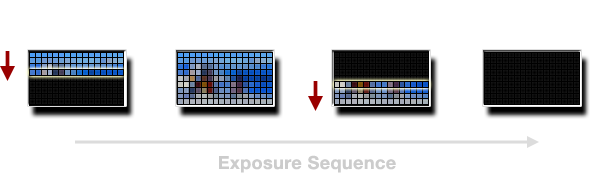
\includegraphics[width=1\linewidth]{assets/rolling-shutter-timeline.png}
        \caption{}
        \label{subfig:rs_timeline}
    \end{subfigure}
    \hfill
    \begin{subfigure}{.49\textwidth}
        \centering
        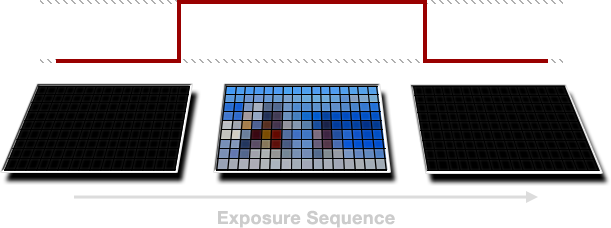
\includegraphics[width=1\linewidth]{assets/global-shutter-timeline.png}
        \caption{}
        \label{subfig:gs_timeline}
    \end{subfigure}
    \hfill
    \begin{subfigure}{0.49\textwidth}
        \centering
        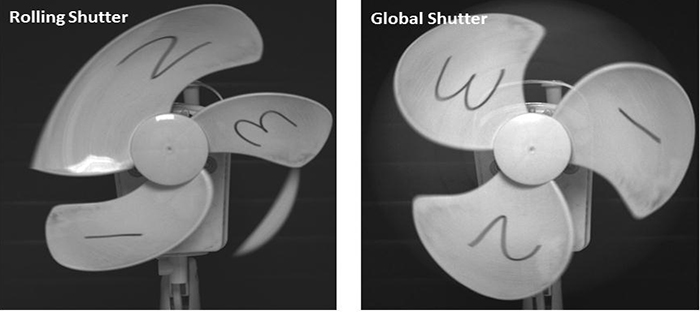
\includegraphics[width=0.7\textwidth]{assets/rolling-vs-global-shutter.jpeg}
        \caption{}
        \label{subfig:rs_vs_gs}
    \end{subfigure}
    \caption{(a) An image capture timeline of a rolling shutter sensor, (b) An image capture timeline of a global shutter sensor \cite{reddigitalcinemaGlobalRollingShutters}, (c) The distortion in the image capture of a spinning fan due to a rolling shutter, compared to a non-distorted capture from a global shutter \cite{RollingShutterVs}.}
    \label{fig:rs_vs_gs}
\end{figure}

The article in \cite{updatedWhatGlobalShutter2021} explains: Instead of having pixels from the top of the sensor switch on and work its way down like a scan, the global shutter sensor takes a snap of the scene using all of the pixels all at once. Figures \ref{subfig:rs_timeline} and \ref{subfig:gs_timeline} illustrate the differences in image capture, and Figure \ref{subfig:rs_vs_gs} illustrates the drastic differences in each shutter type. The Raspberry Pi company produces a global shutter camera featuring a 1.6MP Sony IMX296 sensor, with plug-and-play compatibility with RPi computers \cite{raspberrypiltdBuyRaspberryPib}.

\subsection{Machine Vision Technologies for Backscatter Detection and Tracking}
Underwater backscatter has a mixture of many compositions, from bubbles and sand to all sorts of other marine debris. It is much easier to explore the image processing for one backscatter composition type and later expand to cover all types. Many environmental analysis fields employ systems for underwater bubble quantification to study gas seepages from the sea floor. These systems require implementations of bubble detection to calculate the exact outline and shape with bubble tracking to measure the movement to calculate the volume, flux, and overall chemical composition. Gas escape measurement and monitoring systems require high precision, extensive range, strong anti-interference, and low cost under complex underwater conditions \cite{zhangUnderwaterBubbleEscape2023}. Therefore, research into this field to harness techniques should theoretically provide a boost to help with the accurate backscatter cancellation project aim.

\subsubsection{Automated gas bubble imaging at sea floor - a new method of in situ gas flux quantification \cite{thomanekAutomatedGasBubble2010}}
This paper presents the design of a novel method for automated gas bubble imaging, its validation procedures and calibration experiments, with the primary aim of quantifying gas flux from gas release sites on the sea floor for environmental analysis. The authors have identified two main factors of the system: (a) segmentation by isolating the bubbles from the image background and (b) determining their position and sizes with bubble tracking in successive frames.

\begin{figure}[h]
    \centering
    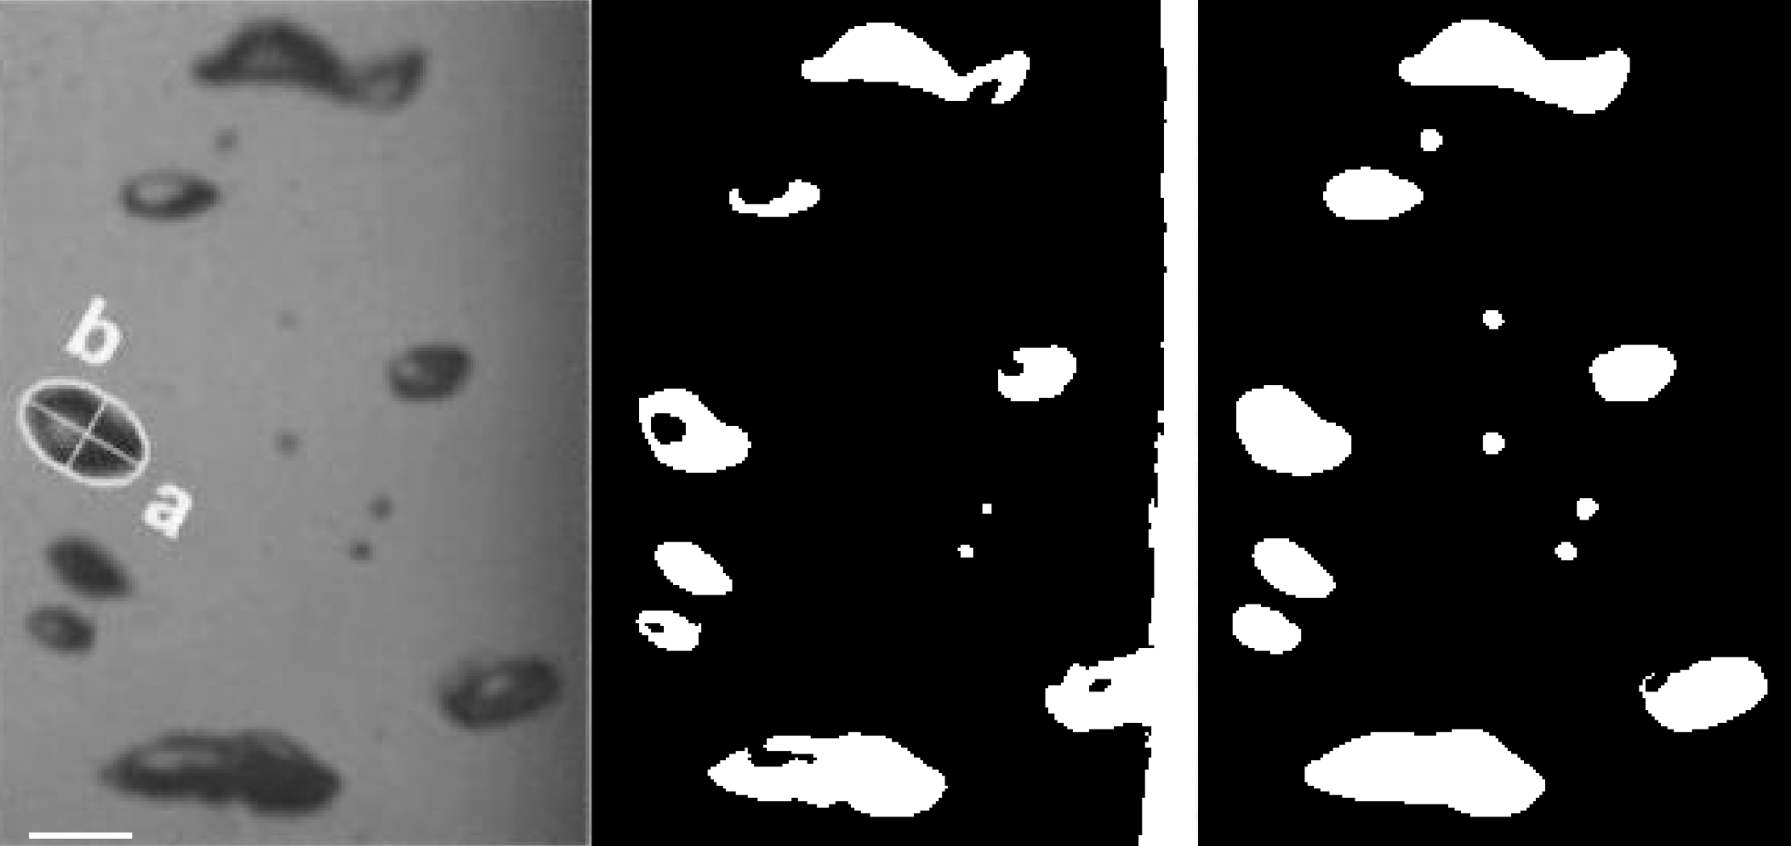
\includegraphics[width=0.65\textwidth]{assets/bubble-segmentation-canny-thresholding.png}
    \caption{An illustration from the paper in \cite{thomanekAutomatedGasBubble2010} showing the original input in the left-most image, bubble segmentation using a simple thresholding method in the middle, and bubble segmentation using Canny in the right-most image.}
    \label{fig:bubble_segment_canny}
\end{figure}

This paper employs the Canny edge detection algorithm \cite{cannyComputationalApproachEdge1986} for greyscale images. The Canny filter compares the value of each pixel relative to its neighbours, so when the gradient between two adjacent pixels is higher than a certain threshold, the algorithm sets the bordering pixel to a value of binary `1', otherwise `0', resulting in the formation of edges around objects. The paper compares the Canny segmentation approach with simple thresholding (blob detection approach) and deduces Canny as more accurate for segmentation, even in inhomogeneously illuminated areas. However, the disadvantages of Canny are the drastic increase in computing time and the requirement for implementing morphological techniques to account for the growing or shrinking of bubbles during segmentation.

The paper outlines a method for bubble tracking using the `least distance' rule, which is the realisation that the distance a bubble travels in two successive frames is smaller than the distance to its closest neighbour. This assumption, although not valid for overlapping bubbles, very high bubble concentrations, and cases where the travel distance exceeds the neighbouring bubble distances, enables a computationally simple method for calculating positions in successive frames and the bubble rise velocity from the sea floor. While this paper explores methodologies perfect for a starting point, it does focus more on the system construction and quantifying gas flux measurements, thus skipping some information on vital aspects such as how the bubbles were perfectly highlighted after Canny in Figure \ref{fig:bubble_segment_canny}, one can assume they are using logic to fill closed loop edges.

\subsubsection{Gas Bubble Shape Measurement and Analysis \cite{zelenkaGasBubbleShape2014}}
Gas bubbles emerging from sea floor seepages rise at high speeds and may change in form, contour, and volume during their ascent. This paper aims to develop robust methods for automated image processing to extract the shape, motion, and volume from a sequence of image frames. The paper mentions the work in \cite{thomanekAutomatedGasBubble2010} to form a baseline. The sporadical false detection characteristic of the Canny edge detector due to light areas inside bubbles derives a motivation to search for more stable algorithms. This paper introduces methods for precise bubble stream quantification and accurate bubble elliptical fitting with snake-based methods, where a snake is an energy-minimising spline guided by external constraint forces and influenced by image forces that pull it towards features such as lines and edges, and the Covariance Matrix Adaptation - Evolution Strategy (CMA-ES) optimisation algorithm, which aids in solving non-linear, non-convex optimisation problems and is particularly effective for continuous optimisation tasks where the objective function may be multimodal, noisy, or complex.

\begin{figure}[h]
    \centering
    \begin{subfigure}{.40\textwidth}
        \centering
        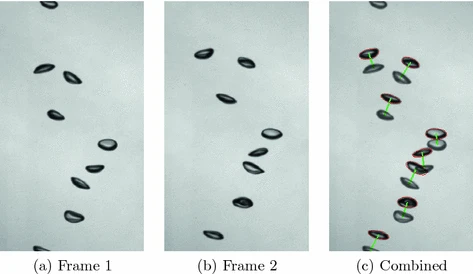
\includegraphics[width=1\linewidth]{assets/zelenkaGasBubbleShape2014-movement_tracking.png}
        \caption{}
        \label{subfig:zelenka_tracking}
    \end{subfigure}
    \hfill
    \begin{subfigure}{.55\textwidth}
        \centering
        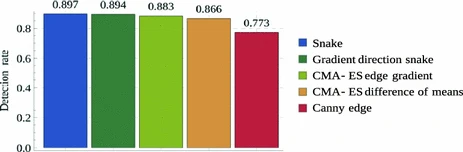
\includegraphics[width=1\linewidth]{assets/zelenkaGasBubbleShape2014-bubble-detection-methods-comparison.png}
        \caption{}
        \label{subfig:zelenka_compare}
    \end{subfigure}
    \caption{From \cite{zelenkaGasBubbleShape2014}: (a) illustration of the movement of bubbles in between two frames at 100 fps. The combination shows frames 1 and 2 with the bubble detection in frame 2 in red and matching bubbles connected in green, (b) a graph comparing the detection rates for several selected methods on a high-quality GoPro image sequence with manual ground truth on 20 images.}
    \label{fig:zelenka}
\end{figure}

The paper implements bubble movement tracking between the current and previous frames using a Kalman filter \cite{kalmanNewApproachLinear1960} to predict the bubble position in a subsequent frame from detection, employing the Hungarian method \cite{kuhnHungarianMethodAssignment1955} for the minimum weighted matching of the predicted positions and the new detection of bubble positions. Figure \ref{subfig:zelenka_tracking} illustrates both the bubble detection and movement tracking between frames, notably observing the precise red border that follows the exact outline of the bubble in addition to the accurate tracking even in bubble-dense regions. The methods this paper explores are compared based on performance, illustrated in Figure \ref{subfig:zelenka_compare}. The standard snake method achieves an 89.7\% decision rate, a 12.4\% advantage over the standalone Canny system.

\subsubsection{The Python Programming Language and OpenCV}
OpenCV is an open-source computer vision and machine learning software library with over 2500 optimised algorithms, including a comprehensive set of classic and state-of-the-art computer vision and machine learning algorithms \cite{opencv}. Although native to C++, OpenCV features interfaces for Python, Java and MATLAB, ensuring compatibility with Windows, Linux, Android, and macOS. OpenCV targets real-time vision applications by taking advantage of CPU accelerators, such as MMX and SSE instructions for parallel data processing, and GPU accelerators, with ongoing development of a full-featured CUDA and OpenGL interface.

\subsection{Real-time Systems}
A real-time operating system (RTOS) enables the compliance of a `hard' real-time system, where there is a guarantee of the maximum time a task requires for completion. An RTOS is typically suited for low-power, embedded systems such as single-core STM32 microcontrollers due to their deterministic behaviour, low-latency interrupt handling, and low-complexity design. However, an STM32 microcontroller cannot handle the high computational requirements of machine vision tasks, thus invoking a preference towards an RPi, such as the Pi 4, or an FPGA-based system. All RPi's non-microcontroller product offerings are RTOS unsuitable due to high system complexity, as confirmed by \cite{FreeRTOSRaspberry2022}. Despite the presence of a FreeRTOS port for the Pi 4 \cite{timadaTImadaRaspi4_freertos2024}, there are many limitations and thus will exponentially increase development times.

\subsubsection{Understanding Linux real-time with PREEMPT\_RT training \cite{bootlinUnderstandingLinuxRealtime2024}}
This piece of literature is a 123-slide training presentation by Bootlin that covers RTOS fundamentals, Linux, and the PREEMPT-RT patch. Most multi-tasking OSes, such as Linux, are pre-emptive, meaning that when a task runs in user space mode and is interrupted and if the interrupt handler can wake up another task, the scheduler will schedule this task as soon as the interrupt handler returns. Since the Linux kernel does not support pre-emption due to the presence of spinlocks rather than mutual exclusion around critical sections, pre-emption logic falls apart when a user-space task calls kernel-specific functions, thus accepting a promotion to kernel-space as it receives an interrupt.

\begin{figure}[h]
    \centering
    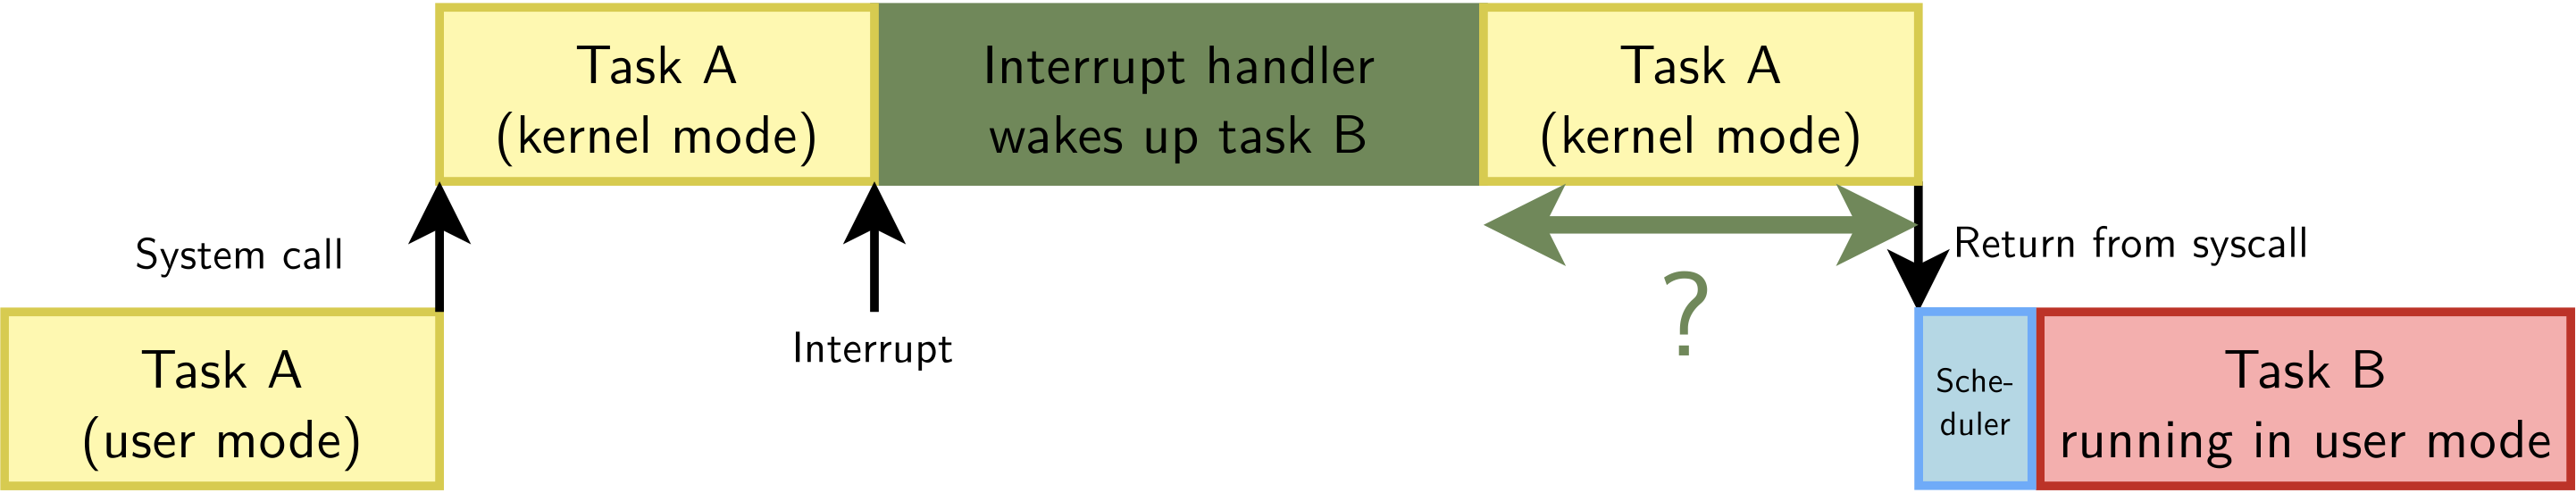
\includegraphics[width=0.65\textwidth]{assets/bootlin-interrupt-flow.png}
    \caption{Illustration of the interrupt flow within two tasks, one in kernel space and another in user space \cite{bootlinUnderstandingLinuxRealtime2024}.}
    \label{fig:bootlin_flow}
\end{figure}

Figure \ref{fig:bootlin_flow} illustrates this issue when a task promotes into kernel space. Critical sections are bound with spinlocks, ultimately preventing the immediate pre-emption of the scheduler by holding Task A to schedule Task B. When the interrupt handler wakes Task B, Task A resumes and will continue until the spinlock completes, resulting in monumental and unpredictable latencies. Aside from the kernel-space incompatibility, Linux already supports user-space pre-emption with task priority-based real-time scheduling to allow for an RTOS. The PREEMPT-RT is a kernel patch that aims to make all kernel-space code preemptible and deterministic. Although insufficient to convert Linux into an RTOS, the PREEMPT-RT patch is a step in the correct direction to minimise task switching latencies. The presentation discusses the limitations of Linux and Linux-compatible hardware with RTOS: Linux will never be a formally proven RTOS, and the hardware Linux typically runs on isn't designed with RT in mind.

\subsubsection{Raspberry Pi 4B: Real-Time System using Preempt-RT (kernel 4.19.y) \cite{maurorivaRaspberryPi4B2019}}
This blog post details the installation steps for the PREEMPT-RT kernel patch in a Raspberry Pi 4 Linux system. The RT-Tests, a test suite that contains programs to test various real-time Linux \cite{costashulRTTests2023}, quantifies the latency reduction with the kernel modification, drawing comparisons with the non-RT kernel.

\begin{figure}[h]
    \centering
    \begin{subfigure}{.44\textwidth}
        \centering
        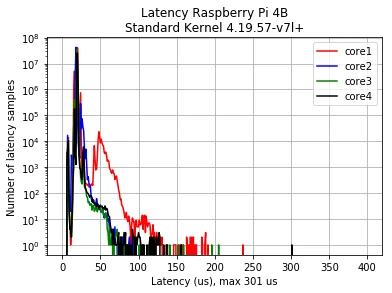
\includegraphics[width=1\linewidth]{assets/lemariva-std-kernel-latency.png}
        \caption{}
        % \label{subfig:std_kernel_latency}
    \end{subfigure}
    \qquad
    \begin{subfigure}{.44\textwidth}
        \centering
        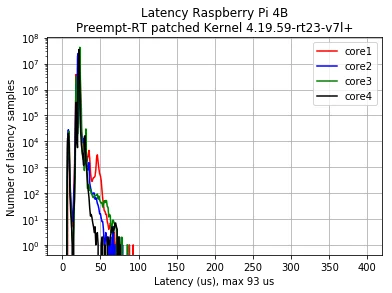
\includegraphics[width=1\linewidth]{assets/lemariva-rt-kernel-latency.png}
        \caption{}
        % \label{subfig:rt_kernel_latency}
    \end{subfigure}
    \caption{Illustration from \cite{maurorivaRaspberryPi4B2019} showing the latency measurements following a Cyclictest execution from the RT-Tests suite for (a) the standard Linux RPi kernel and (b) the PREEMPT-RT patch Linux RPi kernel.}
    \label{fig:lemariva_latency}
\end{figure}

The Cyclictest, part of RT-Tests, accurately and repeatedly measures a thread's intended wake-up time and when it wakes up to provide statistics about the system's latencies, measuring latencies in real-time systems caused by the hardware, the firmware, and the operating system \cite{costashulCyclictest2023}. The maximum latency measurement with the standard kernel was \SI{301}{\micro\second}, while the PREEMPT-RT kernel was \SI{93}{\micro\second}, thus confirming a 3.23x latency reduction using the kernel patch.
